\documentclass[11pt,a4paper]{ctexart}
\usepackage{amsmath,amssymb,bm}
\usepackage{graphicx}
\usepackage{booktabs}
\usepackage{geometry}
\usepackage{caption}
\usepackage{subcaption}
\usepackage{float}
\usepackage{hyperref}
\usepackage{enumitem}
\usepackage{xcolor}
\usepackage{longtable}
\usepackage{url}
\geometry{left=2.2cm,right=2.2cm,top=2.4cm,bottom=2.4cm}
\graphicspath{{figures/}}
\hypersetup{colorlinks=true, linkcolor=blue!45!black, citecolor=blue!45!black, urlcolor=blue!45!black}
\setlist[itemize]{leftmargin=2em,itemsep=0.25em}
\setlist[enumerate]{leftmargin=2em,itemsep=0.25em}
\captionsetup{font=small,labelfont=bf}

\title{EP-FLUX 发展脉络与 Dual-Zone EP 正式诊断口径}
\author{Kuroshiou / S-H-I-T-ocean 项目内部报告}
\date{2026 年 9 月 6 日}

\begin{document}
\maketitle

\begin{abstract}
本文整理从 EP-FLUX 理论引入到 Dual-Zone EP 诊断口径形成的完整过程。核心结论是：在我们的最新 Kuroshiou 代表涡和对象级审计中，倾斜坐标修正是稳健正信号，$|F_z^{\mathrm{tilt\ correction}}|/|F_z^{\mathrm{ordinary}}|$ 的典型量级约为 $0.47$，说明涡轴倾斜会明显改写热/浮力相关的垂向 EP 通量；但 thin curved tube 的一阶 metric/Jacobian/Christoffel 小曲率假设在当前代表涡上失效，$\epsilon_{curvature}=\kappa r$ 的中位量级约为 $10-35$，不能作为强闭合解释。随后，material-volume、object-level LAVD/geodesic 与 PV-retention 审计进一步显示：Hua/LAVD 运动学旋转核与 PV anomaly 动力核心存在系统性分离，强行要求单一材料涡体积同时解释 trapping、heat/PV stirring 和 EP forcing 并不合理。因而本文将正式诊断框架升级为 Dual-Zone：inner material core 负责 trapping/material coherence，PV-active shell 负责主要 stirring 与倾斜修正，exchange layer 单独列账边界 heat/PV/momentum exchange。
\end{abstract}

\tableofcontents
\newpage

\section{问题起点：为什么把代表涡输送放入 EP 框架}

最初的问题并不是为了构造一个新的复杂理论，而是很朴素：我们的代表涡旋已经能给出速度、温度、PV proxy 和热/PV 协方差输送，那么这些量能不能放进一个更接近动力学的框架中解释？传统 heat transport 文献提醒我们，涡旋输送不能用“平均速度乘平均温度”替代，而应当看乘积后平均或协方差，例如 \cite{HausmannCzaja2012,DongEtAl2014}
\begin{equation}
  H^{stir}=\rho_0 C_p\langle v'\theta'\rangle,
\end{equation}
以及
\begin{equation}
  \langle vX\rangle=\langle v\rangle\langle X\rangle+\mathrm{cov}(v,X),\quad X=\theta',q'.
\end{equation}
这也是我们早期 aggregate-product stirring 诊断的核心：先算瞬时或对象级乘积，再平均。

EP flux 和 TEM/PV flux 理论提供了更进一步的解释路径。EP flux 原本用于波-平均流相互作用和 PV 通量闭合 \cite{AndrewsMcIntyre1976,Plumb1985}。在我们的涡旋局地坐标里，若把沿涡旋切向/轴向的速度扰动记为 $u_s'$，法向或径向扰动记为 $u_n'$，浮力扰动记为 $b'$，普通垂向 EP flux 可以写成
\begin{equation}
  F_z^{\mathrm{ordinary}}
  =\rho_0 f_0\frac{\langle u_n'b'\rangle}{N^2}.
\end{equation}
这个式子有一个隐含假设：垂向坐标近似为固定的物理 $z$ 方向，涡旋中心轴没有显著随深度偏移，或者这种偏移对垂向导数影响很小。

然而我们的 Kuroshiou 涡旋不是这种简单对象。Hua 弱速中心线、代表涡轴线和旋转核心诊断都显示：许多涡旋有明显倾斜、间断式层间跳变、月牙状强速带和速度中心/PV 核心分离。因此，第一步自然是问：如果涡轴倾斜，普通垂向 EP flux 是否仍可直接使用？

\section{倾斜坐标 EP：第一个稳定正结果}

\subsection{为什么引入倾斜轴坐标}

当中心轴随深度变化时，沿“涡旋自身坐标”的垂向变化不再等于简单的 $\partial_z$。设涡旋中心线为
\begin{equation}
  \bm r_c(z)=(x_c(z),y_c(z)),
\end{equation}
则沿倾斜轴坐标的垂向导数会包含水平位移项：
\begin{equation}
  \left.\frac{D}{Dz}\right|_{eddy}
  \approx \partial_z
  -\frac{\partial x_c}{\partial z}\partial_x
  -\frac{\partial y_c}{\partial z}\partial_y .
\end{equation}
因此普通垂向 EP flux 需要改写为
\begin{equation}
  F_z^{\mathrm{tilted}}
  =F_z^{\mathrm{ordinary}}+F_z^{\mathrm{tilt\ correction}}.
\end{equation}
这里的 $F_z^{\mathrm{tilt\ correction}}$ 表示由于涡轴倾斜导致的坐标导数修正。它不是额外随意加上的经验项，而是把“垂向导数沿着哪个坐标方向取”说清楚之后自然出现的项。

\subsection{生命周期验证结果}

全生命周期 EP 验证给出了本项目中目前最清楚的正结果：在当前 EP 诊断框架下，倾斜修正不是小量。主口径和对照口径的典型结果显示
\begin{equation}
  \mathrm{median}\left(
  \frac{|F_z^{\mathrm{tilt\ correction}}|}
       {|F_z^{\mathrm{ordinary}}|}
  \right)\approx 0.47,
\end{equation}
四分位范围约为 $0.32-0.62$，个别区域或时相可超过 $1$。这说明若使用倾斜涡旋坐标，热/浮力相关的垂向 EP flux 会被显著改写。

\begin{figure}[H]
  \centering
  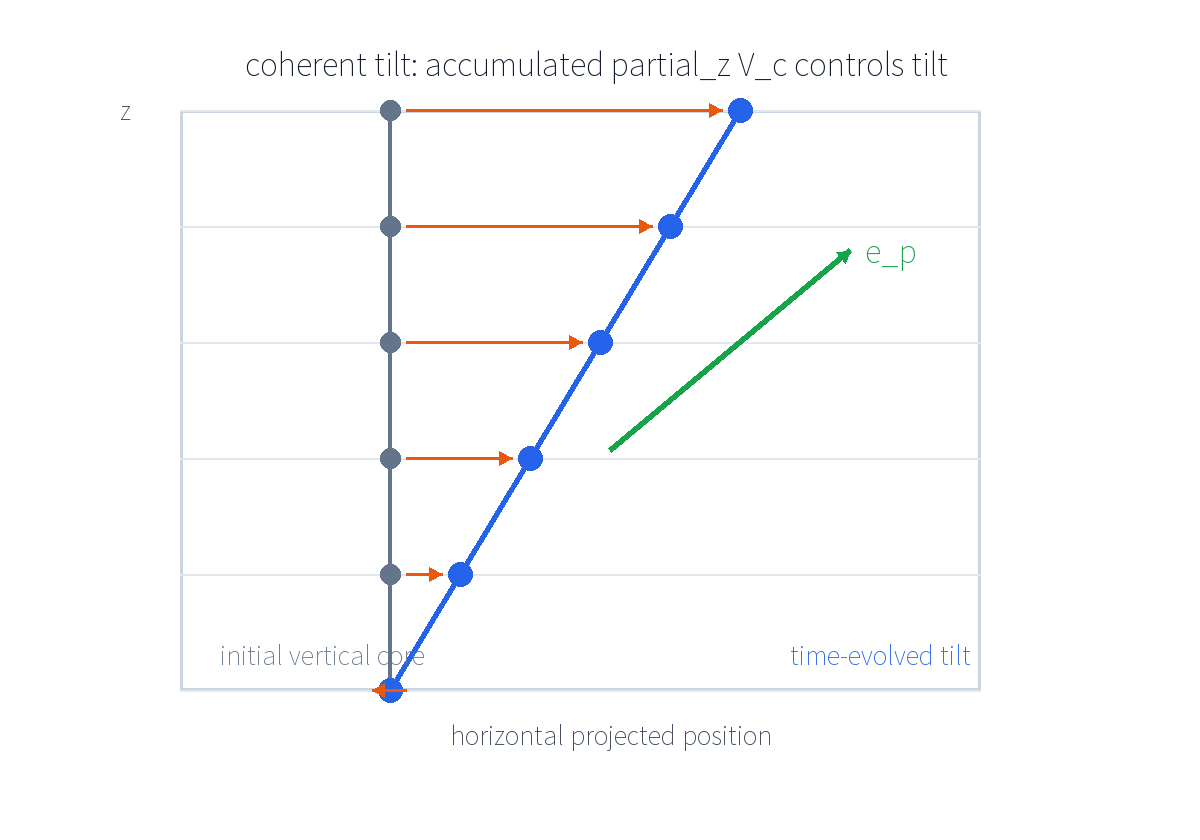
\includegraphics[width=0.88\linewidth]{fig_tilt_correction_lifecycle.png}
  \caption{全生命周期倾斜修正验证图。该图支撑的核心结论是：$|F_z^{\mathrm{tilt\ correction}}|/|F_z^{\mathrm{ordinary}}|$ 不是小量，倾斜轴坐标会改变垂向 EP flux 的量级和空间分布。}
  \label{fig:tilt_lifecycle}
\end{figure}

这一步解决了第一个问题：普通垂向 EP flux 不能无条件当作倾斜涡旋的垂向通量。它也给出了后续工作的基线：不论我们最后使用何种材料边界或分区模型，倾斜修正都必须保留。

\section{Curved-Tube 尝试：为什么不能把曲管几何项当强结论}

\subsection{从倾斜直轴到曲管}

倾斜坐标仍然把涡轴近似成局地直轴。实际代表涡轴线可能是弯曲的，因此我们进一步尝试 curved-tube EP：用沿轴坐标、截面法向坐标和曲率项描述涡旋管。若采用一阶曲管近似，Jacobian 可写为
\begin{equation}
  J=1-\kappa_\alpha x_\alpha,
\end{equation}
其中 $\kappa_\alpha$ 是中心轴曲率在截面方向上的投影，$x_\alpha$ 是截面坐标。相应地，EP 散度会出现 metric、Jacobian 和 Christoffel 类修正项：
\begin{equation}
  \nabla_a F^{ai}
  \sim J^{-1}\partial_a(JF^{ai})+\Gamma^i_{ka}F^{ak}.
\end{equation}

\subsection{失败原因：小曲率条件不成立}

曲管路线的物理直觉是合理的，但一阶 thin curved tube 近似需要
\begin{equation}
  \epsilon_{curvature}=\kappa r \ll 1.
\end{equation}
我们的 metric audit 显示，所有组合的 $\mathrm{metric\_valid\_fraction\_median}=0$，而 $\epsilon_{curvature}$ 的中位量级约为 $10-35$。这远超小曲率近似的适用范围。

\begin{figure}[H]
  \centering
  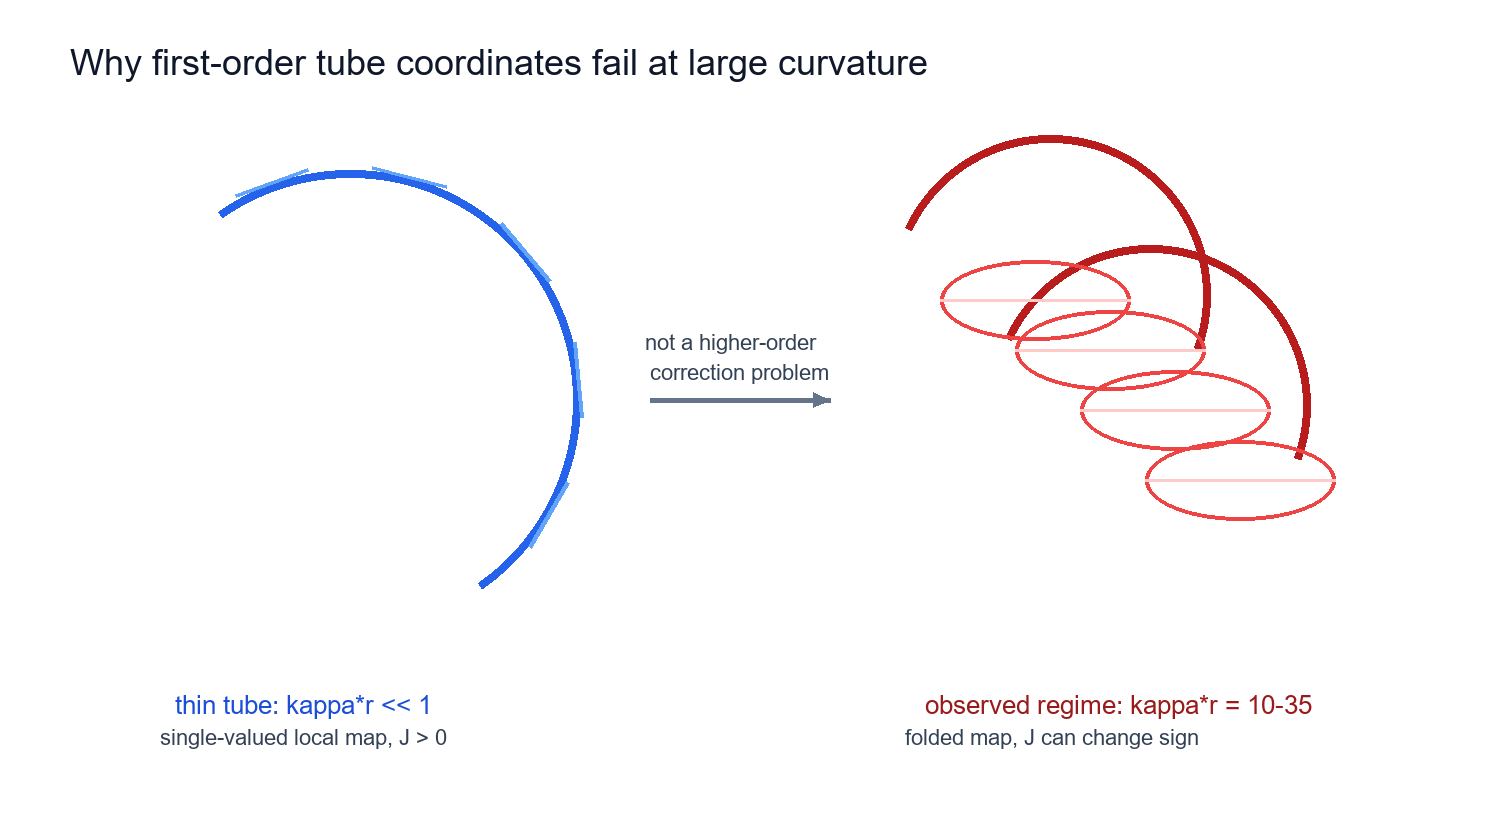
\includegraphics[width=0.85\linewidth]{fig_curvature_failure.png}
  \caption{Curved-tube 小曲率审计。结果显示 $\kappa r$ 过大且 metric 有效比例接近零，因此一阶 Jacobian/Christoffel 不能被写成已经闭合的物理 forcing。}
  \label{fig:curvature_failure}
\end{figure}

因此这一步的结论是负结果，但非常重要：曲管几何项可以作为“为什么需要更复杂几何”的尺度审计，却不能在当前代表涡上作为强闭合解释。我们不能为了理论形式漂亮而忽略适用条件。

\section{Material-Volume 路线：从坐标几何转向体积边界}

\subsection{为什么转向 Cartesian material volume}

当 thin curved tube 失败后，下一步不是继续调 Jacobian，而是换问题表述：既然曲率太大，那就不要强行把涡旋塞进小曲率曲管坐标，而是在 Cartesian 空间里直接寻找一个材料体积。这个思路与 Lagrangian coherent vortex 和材料边界理论更接近 \cite{HallerBeronVera2013,HallerEtAl2016,AbernatheyHaller2018}。

我们依次尝试了 threshold mask、active contour、level set、真实时间 lagrangian boundary，以及完整 3D boundary budget。完整边界预算把侧壁、顶面和底面分开列账：
\begin{align}
  &\oint u_n\,dS,\quad \oint |u_n|\,dS,\\
  &\oint \rho_0 C_p\theta' u_n\,dS,\quad
    \oint q'u_n\,dS,\quad
    \oint b'u_n\,dS,\quad
    \oint u_i'u_n\,dS.
\end{align}
顶/底通量中的 $w$ 仍是连续方程诊断代理，因此报告中一直把它标记为 proxy，而不是直接观测垂直速度。

\subsection{代表涡材料体闭合的限制}

Material-volume 路线带来的第一个教训是：代表涡是平均结构，本身不一定是严格材料体。即使通过边界优化降低泄漏，代表涡层面的 leakage 仍不为零，典型量级约为 $0.018-0.023\,\mathrm{m\,s^{-1}}$。这说明“单一材料体闭合”不能直接建立在平均代表涡上。

\begin{figure}[H]
  \centering
  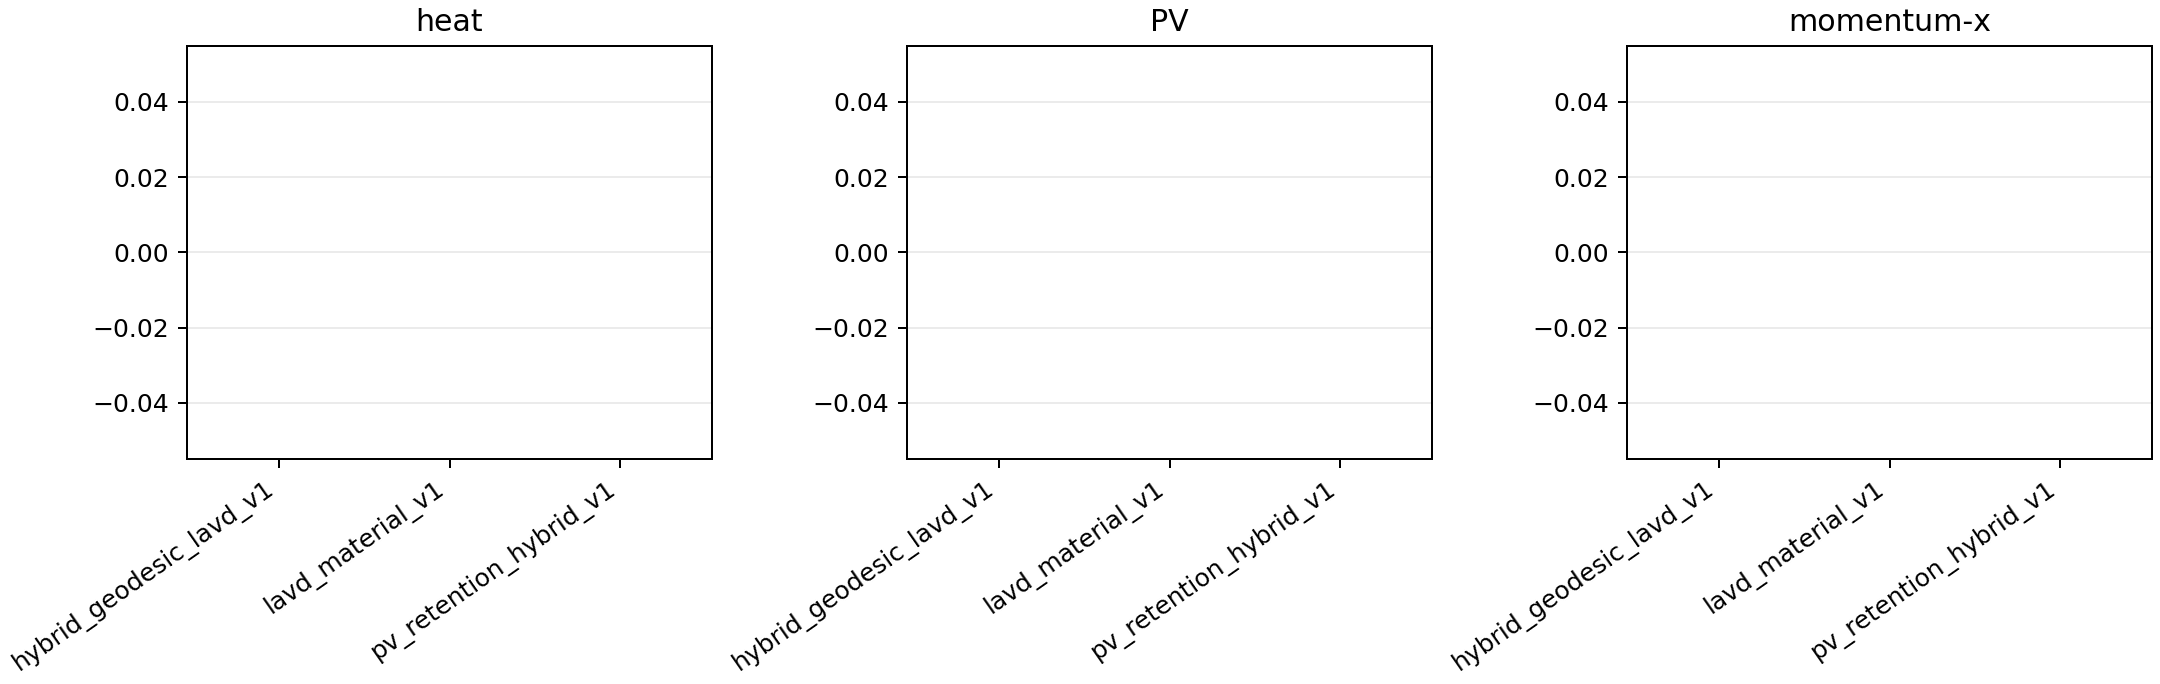
\includegraphics[width=0.86\linewidth]{fig_heat_pv_momentum_budget.png}
  \caption{Object-level 中等样本中的 heat/PV/momentum boundary budget。边界交换不能忽略，因此必须与内部 EP forcing 分开列账。}
  \label{fig:boundary_budget_medium}
\end{figure}

这一步推动我们从代表涡平均场走向 object-level 审计：要判断材料闭合，必须在真实 track/object-day 上看边界随时间的保留、泄漏和交换。

\section{Object-Level LAVD/Geodesic/PV-Retention 审计}

\subsection{三类中心/核心不是同一个物理对象}

object-level 审计迫使我们把“中心”拆开。当前至少有三类核心：
\begin{itemize}
  \item Hua 弱速中心：二维速度弱核并满足旋转几何约束，是我们的识别中心。
  \item LAVD 旋转相干中心：有限时间涡度偏差积分定义的旋转相干材料核中心 \cite{HallerEtAl2016}。
  \item PV anomaly core：PV 异常或 PV 梯度相关的动力核心，更直接对应动力约束和 PV stirring。
\end{itemize}
审计结果显示，Hua 与 LAVD 通常较接近，但 PV core 存在系统性偏离。这意味着速度旋转核和 PV 动力核不能被默认合并。

\begin{figure}[H]
  \centering
  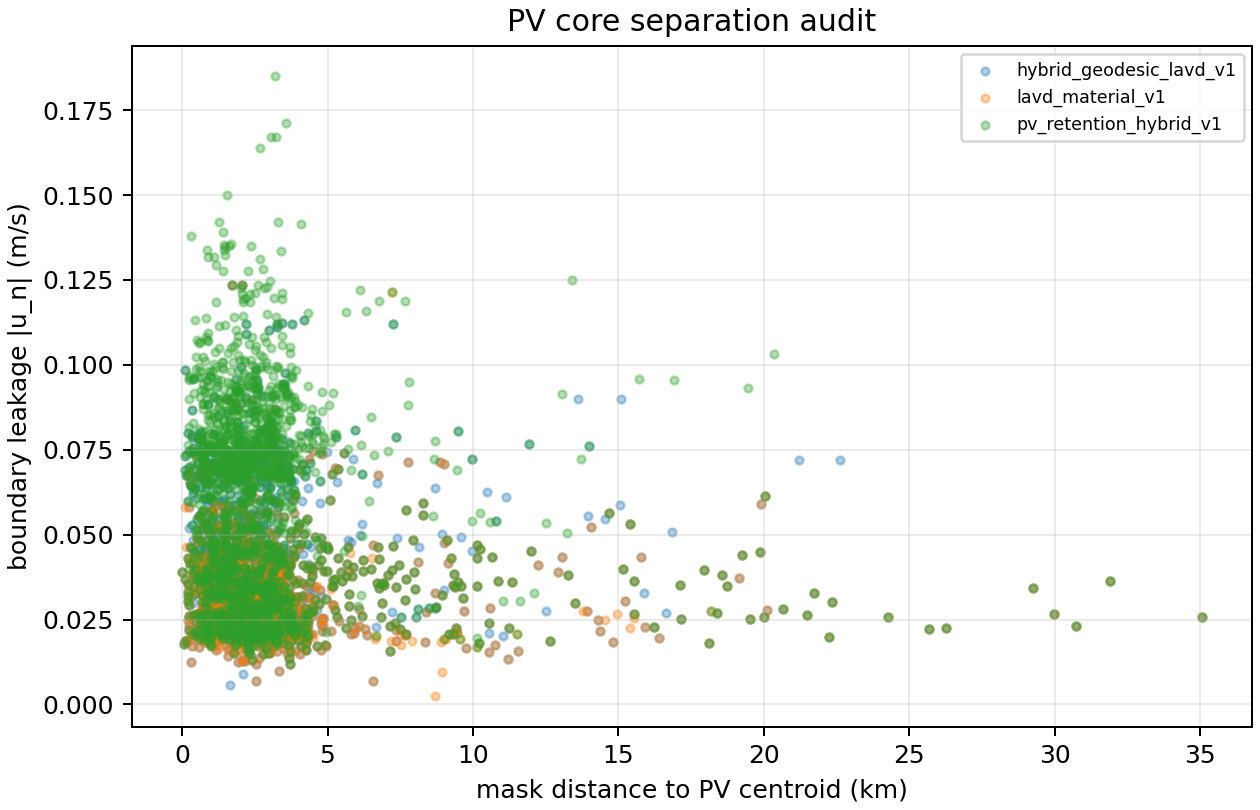
\includegraphics[width=0.82\linewidth]{fig_hua_lavd_pv_separation.png}
  \caption{Hua 弱速中心、LAVD 旋转相干中心与 PV anomaly core 的分离审计。Hua/LAVD 更接近，PV core 更容易偏离，支持“运动学旋转核”和“动力 PV 核”分离。}
  \label{fig:center_separation}
\end{figure}

\subsection{PV-retention 与 leakage 的 tradeoff}

随后我们把 PV retention 从弱评分项升级为主约束。结果并不是简单地“PV retention 提高，闭合就变好”。中等样本显示，PV-retention hybrid 的确提高了 PV core retention，但 leakage、boundary/internal ratio 和 closure residual 往往同步变差。例如 coherent 样本中，PV core retention 从约 $0.064$ 提高到约 $0.142$，但 leakage 从约 $0.0233\,\mathrm{m\,s^{-1}}$ 增加到约 $0.0288\,\mathrm{m\,s^{-1}}$；upright\_like 中也出现类似 tradeoff。

\begin{figure}[H]
  \centering
  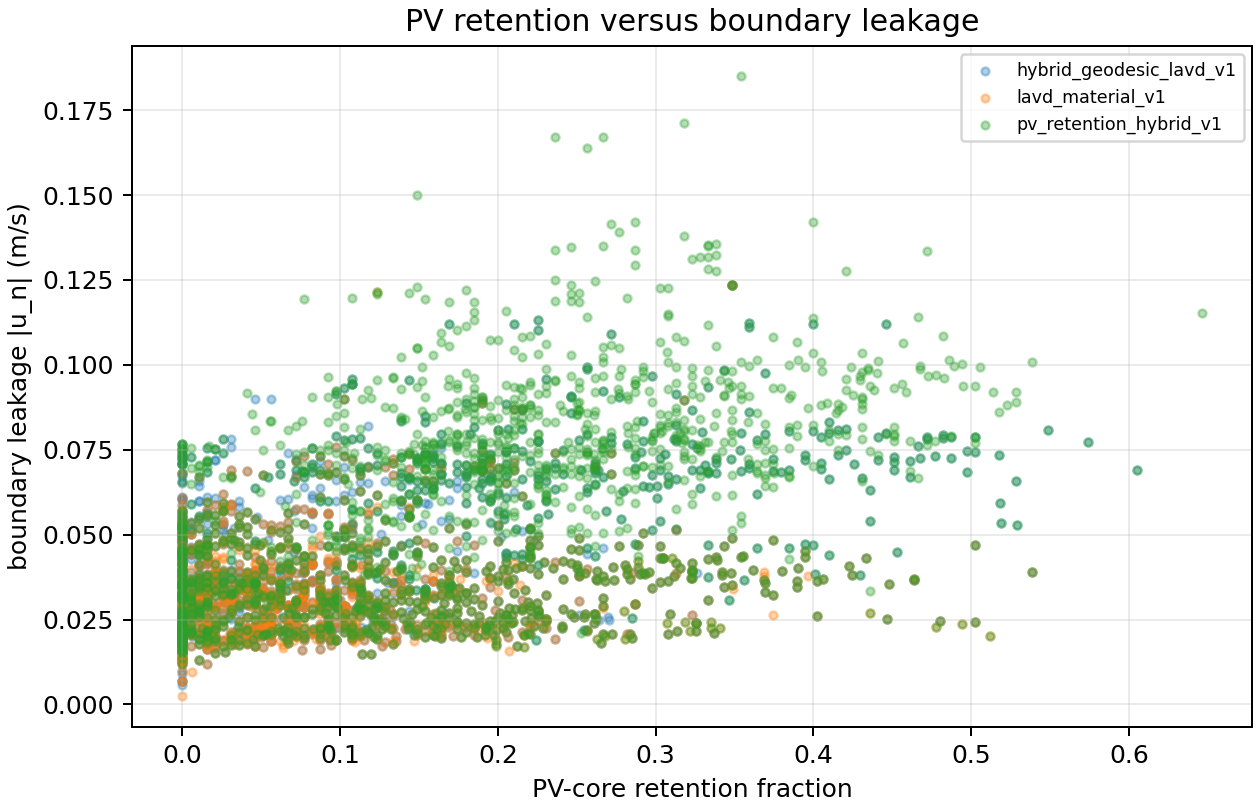
\includegraphics[width=0.86\linewidth]{fig_pv_retention_vs_leakage.png}
  \caption{PV retention 与 leakage 的 tradeoff。提高 PV core retention 往往需要扩大或移动边界，从而增加泄漏和边界交换。}
  \label{fig:pv_retention_leakage}
\end{figure}

\begin{figure}[H]
  \centering
  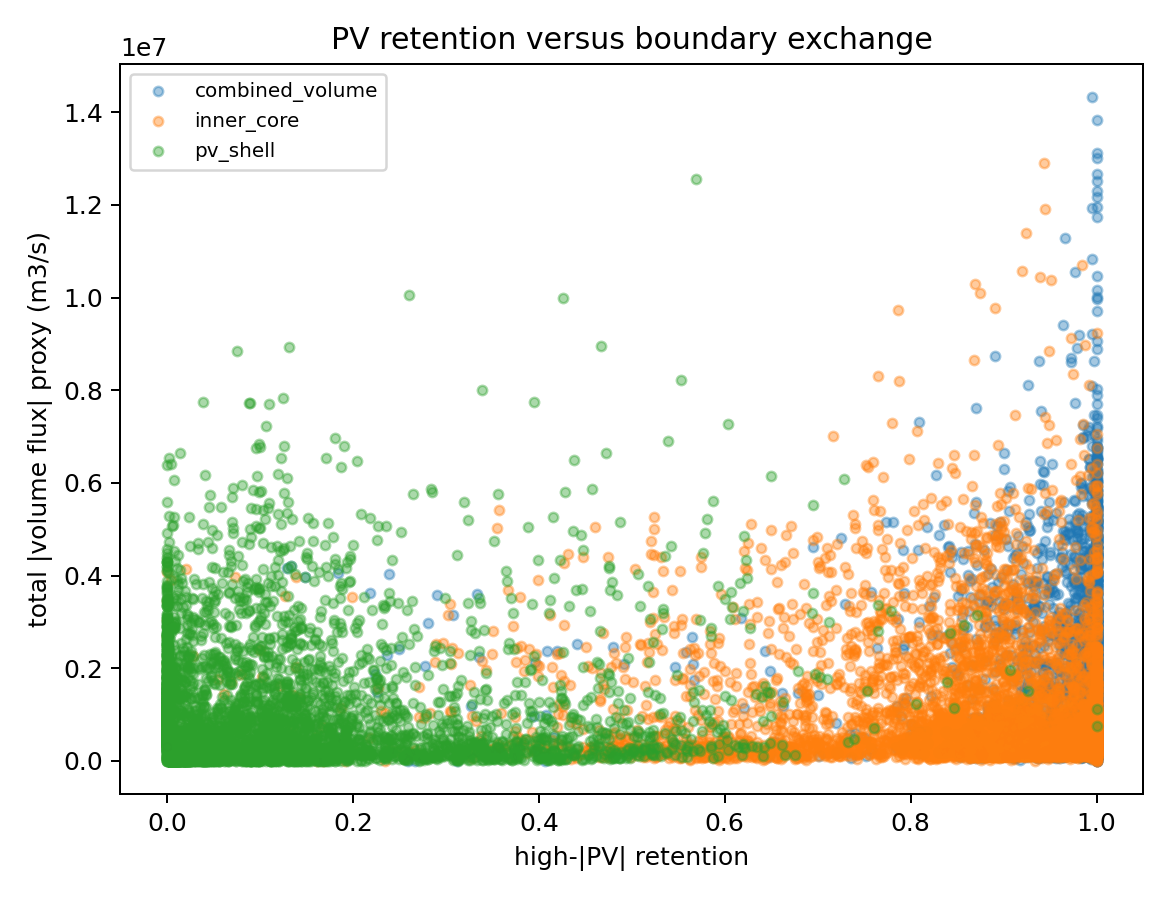
\includegraphics[width=0.86\linewidth]{fig_pv_retention_vs_boundary_exchange.png}
  \caption{PV retention 与 boundary exchange 对照。该图支持一个关键判断：PV-active 区域并不总在低泄漏 LAVD/material core 内部。}
  \label{fig:pv_boundary_exchange}
\end{figure}

这一步给出核心判断：EP 闭合失败不应简单归咎于公式错误，也不应强行要求
\begin{equation}
  PV\ core\subset M_{LAVD}.
\end{equation}
更合理的解释是：低泄漏旋转材料核与 PV-active 动力壳层本来就是两个相邻但不完全重合的区域。

\section{Dual-Zone：从单一材料体闭合升级为分区输送}

\subsection{为什么必须分区}

前面的结果共同指向同一个结论：一个单一边界很难同时满足三件事：低 leakage、高 LAVD/geodesic material coherence、以及高 PV core retention。若强行让材料边界围住 PV core，边界交换会增大；若优先最小化 leakage，PV retention 又偏低。这不是简单调参问题，而是结构分区问题。

因此我们把正式诊断框架改为
\begin{equation}
  \mathcal{T}_{total}
  =\mathcal{T}_{core}^{trap}
  +\mathcal{T}_{shell}^{stir}
  +\mathcal{T}_{exchange}.
\end{equation}
其中：
\begin{itemize}
  \item inner material core：Hua/LAVD 近同位、低 leakage、高 particle retention、弱速核心连通，解释 trapping/material coherence。
  \item PV-active shell：位于 inner core 外侧，高 $|q'|$、高 $|\nabla q'|$、强速度剪切或月牙强速带，解释 heat/PV stirring 和 EP tilt correction。
  \item exchange layer：inner core 与 shell 的接触带，单独计算 heat/PV/momentum boundary exchange。
\end{itemize}

\begin{figure}[H]
  \centering
  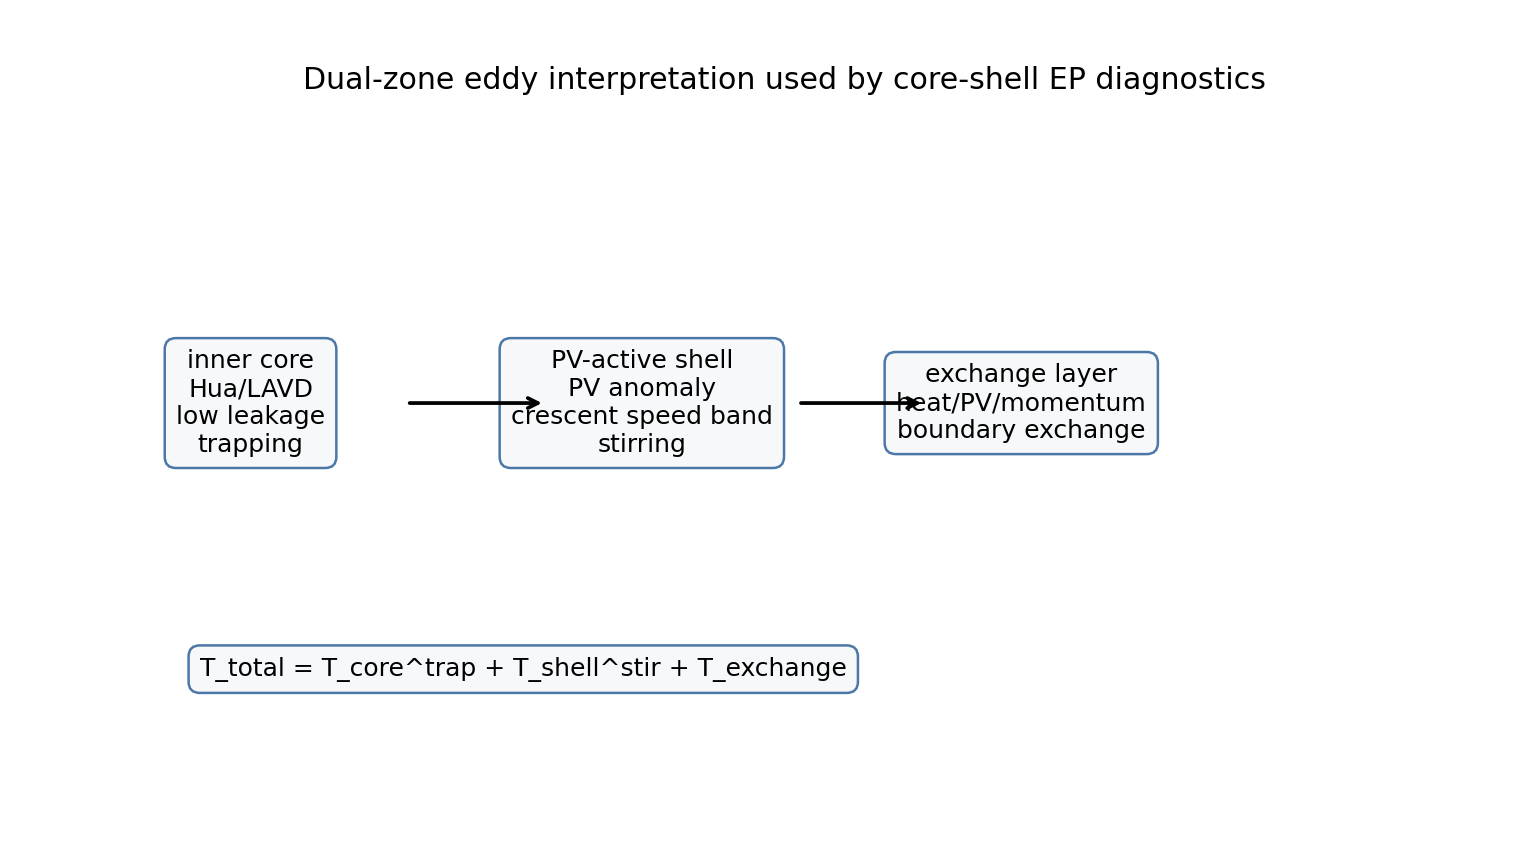
\includegraphics[width=0.9\linewidth]{fig_dual_zone_framework.png}
  \caption{Dual-Zone EP 诊断框架。inner material core 解释 trapping，PV-active shell 解释 stirring，exchange layer 单独列账边界交换。}
  \label{fig:dual_zone_framework}
\end{figure}

\subsection{热/PV stirring 的分区}

Core-Shell V2 进一步把 aggregate-product stirring 放进区域 mask：
\begin{equation}
  H_M=\rho_0 C_p\langle v_{rot}'\theta'\rangle_M,
  \qquad
  P_M=\langle v_{rot}'q'\rangle_M,
\end{equation}
并分别保存 product-mean、mean-product 与 covariance：
\begin{equation}
  \mathrm{cov}_M(v,X)=\langle vX\rangle_M-\langle v\rangle_M\langle X\rangle_M.
\end{equation}
结果显示，PV stirring 更偏向 PV-active shell；heat stirring 在 coherent 中可能接近 core/shell 分担，但在 upright\_like 中更偏 shell。这与 eddy heat transport 和 PV transport 文献中的 core/periphery 区分相吻合 \cite{AbernatheyHaller2018,ZhangWolfeAbernathey2019}。

\begin{figure}[H]
  \centering
  \begin{subfigure}{0.48\linewidth}
    \centering
    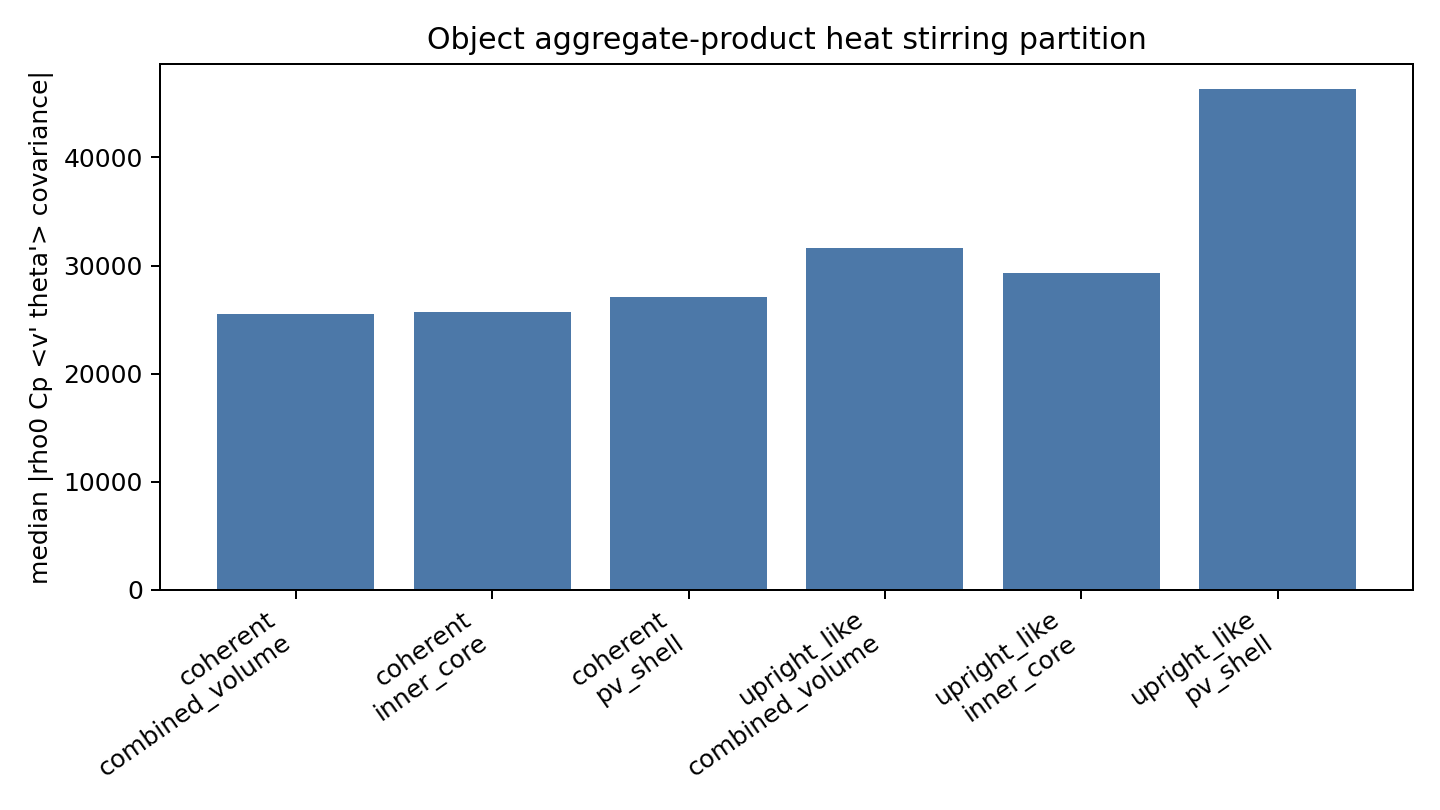
\includegraphics[width=\linewidth]{fig_heat_core_shell.png}
    \caption{Heat covariance partition}
  \end{subfigure}
  \hfill
  \begin{subfigure}{0.48\linewidth}
    \centering
    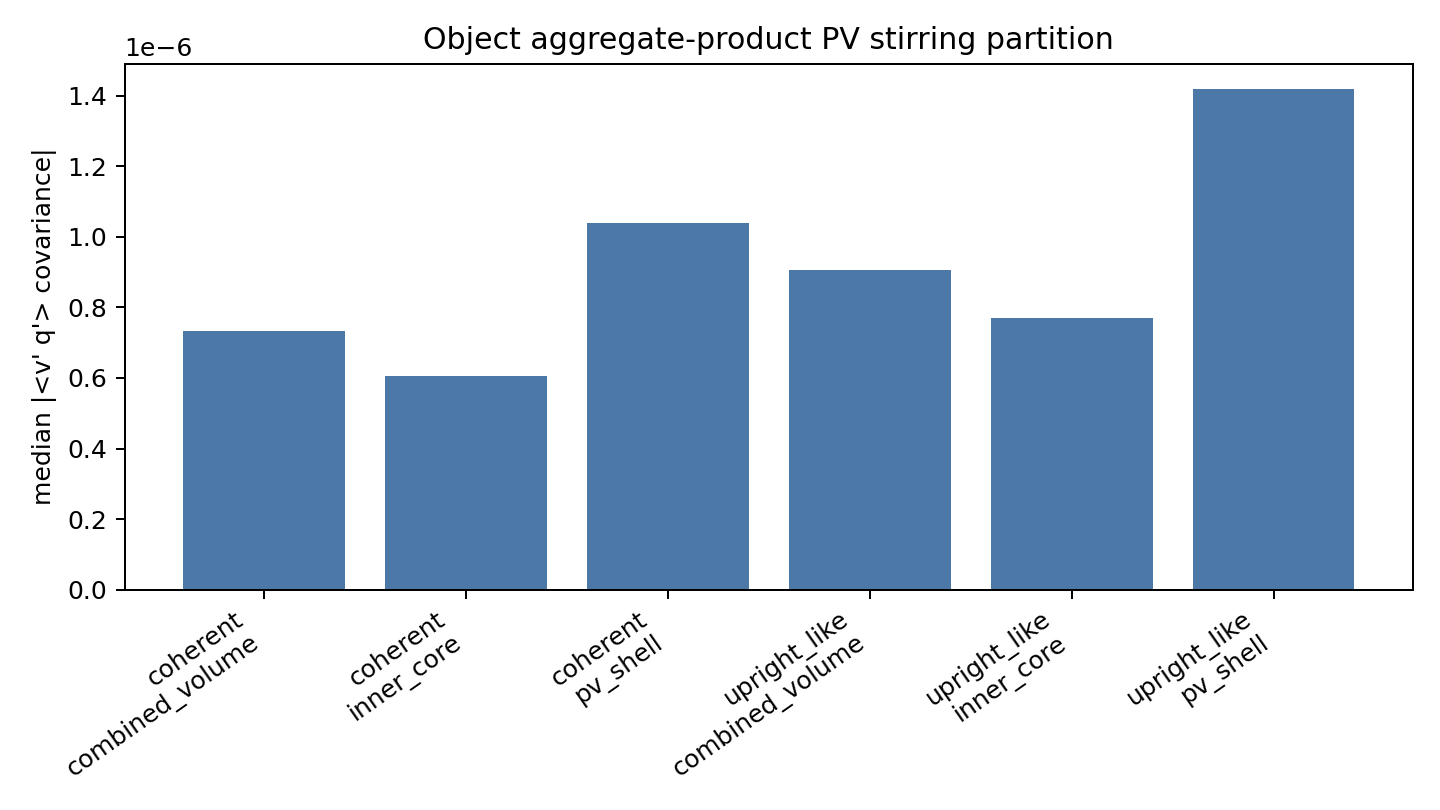
\includegraphics[width=\linewidth]{fig_pv_core_shell.png}
    \caption{PV covariance partition}
  \end{subfigure}
  \caption{热/PV stirring 的 core-shell 分区。PV 通量更明显偏 shell，说明 PV-active shell 是动力搅拌的重要区域。}
  \label{fig:heat_pv_partition}
\end{figure}

\subsection{EP 倾斜修正的分区}

EP 倾斜修正也可以分区写成
\begin{equation}
  F_{z,M}^{\mathrm{tilted}}
  =F_{z,M}^{\mathrm{ordinary}}
  +F_{z,M}^{\mathrm{tilt\ correction}},
\end{equation}
并比较各区贡献比例。V2 结果表明，倾斜修正的重要部分同样偏向 shell 或 core-shell 接触区域，而不是只发生在最内侧材料核。

\begin{figure}[H]
  \centering
  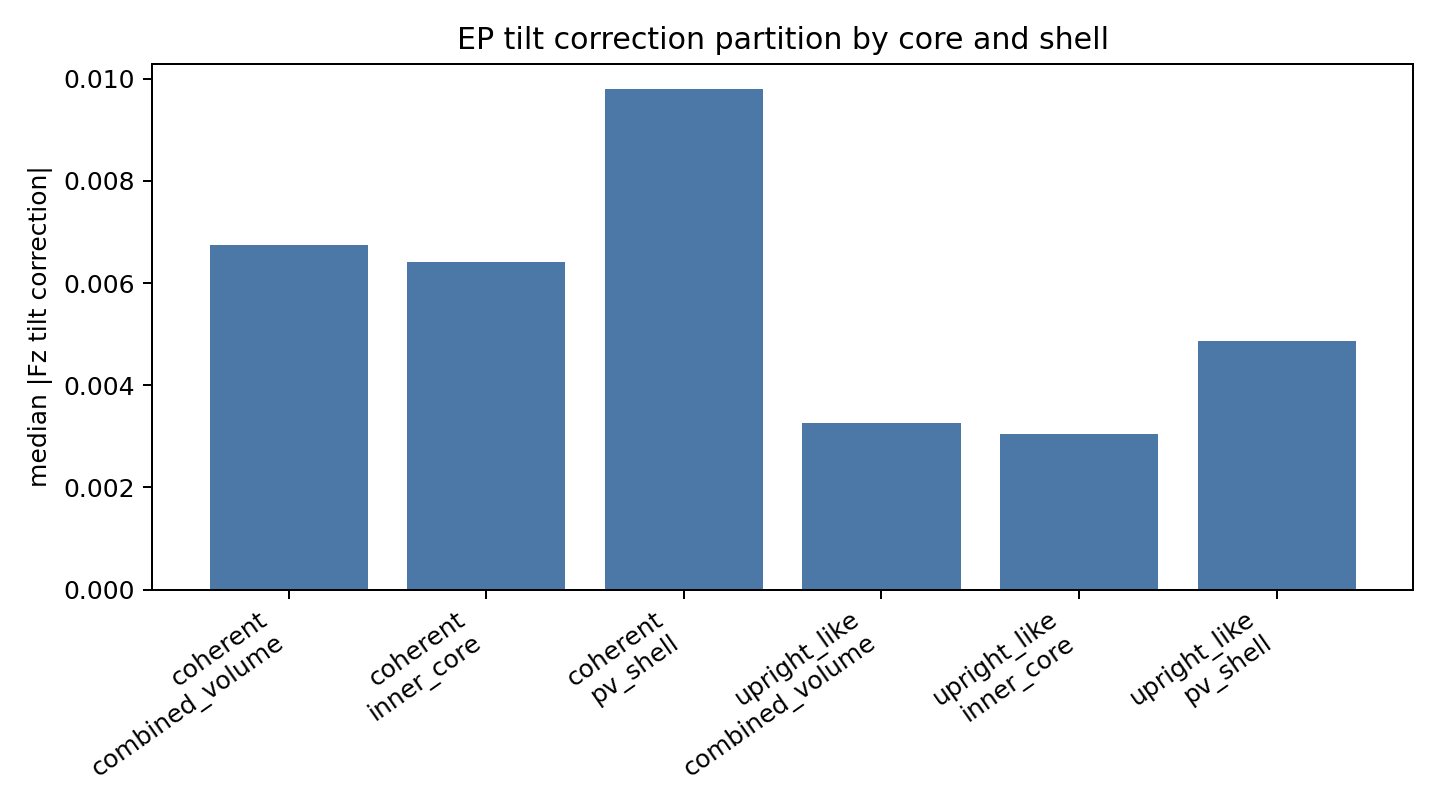
\includegraphics[width=0.88\linewidth]{fig_ep_tilt_core_shell.png}
  \caption{EP tilt correction 的 core-shell 分区。倾斜修正与 PV-active shell 和交换带联系更强，支持 Dual-Zone 而不是单一材料体解释。}
  \label{fig:ep_tilt_partition}
\end{figure}

\subsection{Exchange layer 必须单独列账}

如果 shell 是主要 stirring 区，那么 inner core 与 shell 之间的边界交换就不能被吞进“内部 EP forcing”。我们因此把 heat/PV/momentum boundary exchange 单独输出。

\begin{figure}[H]
  \centering
  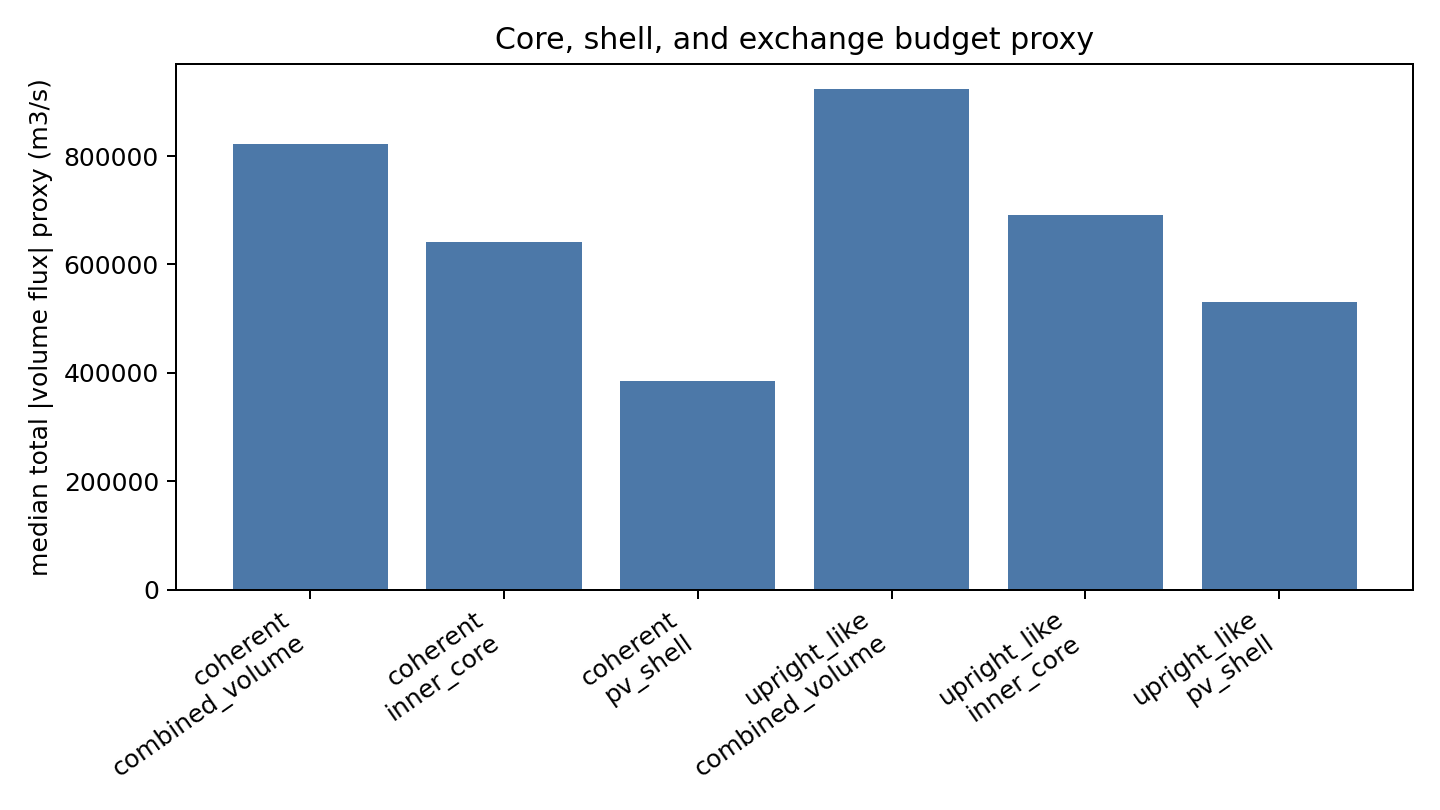
\includegraphics[width=0.88\linewidth]{fig_boundary_exchange.png}
  \caption{Core-shell exchange budget。该图体现 exchange layer 的物理角色：它不是误差项，而是材料核与 PV-active shell 之间真实交换的诊断账户。}
  \label{fig:exchange_budget}
\end{figure}

\section{最终结论与下一步}

\subsection{当前可以稳健写下的结论}

基于从 smoke、代表涡全生命周期、Core-Shell V2 到 object-level medium audit 的证据链，当前结论可以分为四层：
\begin{enumerate}
  \item 倾斜修正是稳健正结果。$|F_z^{\mathrm{tilt\ correction}}|/|F_z^{\mathrm{ordinary}}|$ 的典型量级约 $0.47$，说明倾斜坐标会显著改写热/浮力相关垂向 EP flux。
  \item Thin curved tube 几何不能强解释。$\mathrm{metric\_valid\_fraction\_median}=0$，$\epsilon_{curvature}=\kappa r$ 中位量级约 $10-35$，一阶小曲率近似不成立。
  \item 单一材料涡体积闭合不足。代表涡 leakage 不为零，object-level PV-retention 提高时 leakage/boundary exchange 常变差，说明 PV core 不必属于低泄漏 LAVD core。
  \item Dual-Zone 框架更符合当前证据。inner material core 负责 trapping/material coherence；PV-active shell 负责 heat/PV stirring、月牙强速带和 EP tilt correction；exchange layer 负责边界 heat/PV/momentum exchange。
\end{enumerate}

\subsection{证据等级说明}

这里必须区分不同结果的证据等级：
\begin{itemize}
  \item 全生命周期代表涡验证：支持“倾斜修正不是小量”和“曲管小曲率失败”。
  \item Core-Shell V2 代表涡/object aggregate：支持“PV stirring 与 EP tilt correction 偏 shell”。
  \item object-level medium sample：支持“PV retention 与 leakage 存在 tradeoff”，但还不是全 object-level 统计终局。
\end{itemize}
因此报告不把 medium sample 写成全量结论，也不把 proxy 边界预算写成严格观测闭合。

\subsection{建议采用的正式诊断入口}

后续正式 EP 诊断建议使用
\begin{center}
\texttt{python -m src.EP.cli run-dual-zone-ep-diagnostics}
\end{center}
作为默认解释入口。Single material volume、LAVD/geodesic/PV-retention 边界仍保留为审计工具，用来回答“材料核是否稳定”和“PV core 是否被边界包住”，但不再作为唯一闭合目标。

下一步优先级如下：
\begin{enumerate}
  \item 扩大 object-level medium sample 至更多 track，检验 PV-retention--leakage tradeoff 是否稳定。
  \item 对 heat/PV/momentum boundary exchange 按 shape、polarity、depth 和 tau 分层列账。
  \item 若 tradeoff 稳定，则把 Dual-Zone 写入正式科学口径；若某类涡旋能同时低 leakage 和高 PV retention，则单独标记为强材料闭合特例。
\end{enumerate}

\section*{项目内文件索引}
\begin{itemize}
  \item 本报告目录：\texttt{EP-FLUX/ep\_flux\_development\_history\_report/}
  \item 早期理论：\texttt{EP-FLUX/E-P\_flux理论整理.pdf}
  \item 曲管理论：\texttt{EP-FLUX/curved\_tube\_ep\_flux.pdf}
  \item 大曲率材料体理论：\texttt{EP-FLUX/large\_curvature\_material\_volume\_ep\_flux.pdf}
  \item Core-Shell V2 报告：\texttt{EP-FLUX/core\_shell\_partition\_v2/core\_shell\_partition\_v2\_report\_zh.pdf}
\end{itemize}


\section*{DOI 与链接索引}
\begin{itemize}
  \item Andrews \& McIntyre 1976: \href{https://doi.org/10.1175/1520-0469(1976)033<2031:PWIHAV>2.0.CO;2}{10.1175/1520-0469(1976)033<2031:PWIHAV>2.0.CO;2}
  \item Plumb 1985: \href{https://doi.org/10.1175/1520-0469(1985)042<0217:OTTDPO>2.0.CO;2}{10.1175/1520-0469(1985)042<0217:OTTDPO>2.0.CO;2}
  \item Haller \& Beron-Vera 2013: \href{https://doi.org/10.1017/jfm.2013.391}{10.1017/jfm.2013.391}
  \item Haller et al. 2016: \href{https://doi.org/10.1017/jfm.2016.151}{10.1017/jfm.2016.151}
  \item Abernathey \& Haller 2018: \href{https://doi.org/10.1175/JPO-D-17-0102.1}{10.1175/JPO-D-17-0102.1}
  \item Chelton et al. 2011: \href{https://doi.org/10.1016/j.pocean.2011.01.002}{10.1016/j.pocean.2011.01.002}
  \item Hausmann \& Czaja 2012: \href{https://doi.org/10.1016/j.dsr.2012.08.005}{10.1016/j.dsr.2012.08.005}
  \item Dong et al. 2014: \href{https://doi.org/10.1038/ncomms4294}{10.1038/ncomms4294}
  \item Zhang, Wolfe \& Abernathey 2019: \href{https://arxiv.org/abs/1911.01520}{arXiv:1911.01520}
\end{itemize}

\bibliographystyle{plain}
\bibliography{references}

\end{document}
